\documentclass[tikz,border=5mm]{standalone}

\begin{document}

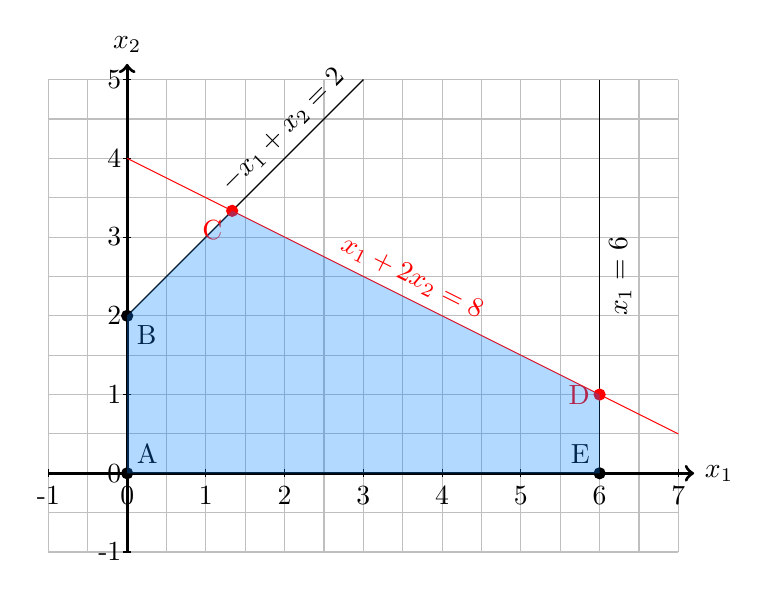
\begin{tikzpicture}

    \draw[gray!50, thin, step=0.5] (-1,-1) grid (7,5);
    \draw[very thick,->] (-1,0) -- (7.2,0) node[right] {$x_1$};
    \draw[very thick,->] (0,-1) -- (0,5.2) node[above] {$x_2$};

    \foreach \x in {-1,...,7} \draw (\x,0.05) -- (\x,-0.05) node[below] {\x};
    \foreach \y in {-1,...,5} \draw (-0.05,\y) -- (0.05,\y) node[left] {\y};

    \draw (0,2) -- (4/3,10/3) -- node[above,sloped] {$-x_1+x_2=2$}  (3,5);
    \draw[red] (0,4) -- node[above, sloped] {$x_1+2x_2=8$} (7,0.5);
    \draw (6,0) -- node[below,sloped] {$x_1=6$} (6,5);
%    \draw[dashed] (5,7) -- node[above right,sloped] {$max\, Z=3x_1+x_2$} (7,1);

    \filldraw [black] (0,0) circle (2pt) node[above right] {A};
    \filldraw [black] (0,2) circle (2pt) node[below right] {B};
    \filldraw [red] (4/3,10/3) circle (2pt) node[below left] {C};
    \filldraw [red] (6,1) circle (2pt) node[left] {D};
    \filldraw [black] (6,0) circle (2pt) node[above left] {E};

    \fill[blue!50!cyan,opacity=0.3] (0,0) -- (0,2) -- (4/3,10/3) -- (6,1) -- (6,0) -- (0,0);

\end{tikzpicture}

\end{document}
